\chapter{Orbit Tomography}\label{chap:orbit_tomography}

%Figure \ref{fig:orbit_fida_spectra}d shows how different spatial locations are weighted by the orbits.
In this chapter we develop Orbit Tomography, a method that uses orbit weight functions to infer the full fast-ion distribution function from experimental measurements.

Recall from Chapter \ref{chap:weights} that the forward model of a diagnostic can be linearized into the following form,
\begin{equation}\label{eq:S_linear}
    s = \sum_k n_k w(\mathbf{J}_k) \;,
\end{equation}
where $s$ is the diagnostic signal, $n_k$ is the number of fast ions on the k$^{th}$ orbit, and $w(\mathbf{J}_k)$ is the orbit's weight function.
In the infinite limit, Equation \ref{eq:S_linear} is an exact representation of the diagnostic's forward model. Truncating the number of orbits reduces the accuracy of the representation but allows for the forward model to be discretized,
\begin{equation}
    s = \mathbf{w}^T\cdot\mathbf{n}\,,
\end{equation}
where each element of $\mathbf{w}$ and $\mathbf{n}$ is the orbit weight function and number of fast-ions on the orbit, respectively. When multiple measurements are available, they can be combined to form a system of linear equations,
\begin{equation}\label{eq:Wxn}
    \mathbf{s} = \mathbf{W}\cdot\mathbf{n}\,,
\end{equation}
where each row of $\mathbf{W}$ contains the weight vector, $\mathbf{w}^T$, for each measurement. Similar to Velocity-space Tomography, the system of linear equations can be solved for the number of fast ions on each orbit, $\mathbf{n}$. Since orbit weight functions are used, instead of velocity-space weight functions, we call the process of solving the system Orbit Tomography.
In addition to the increased fidelity of the linearized forward model, Orbit Tomography has several other advantages over Velocity-space Tomography.

\begin{figure}[h!]
    \centering
    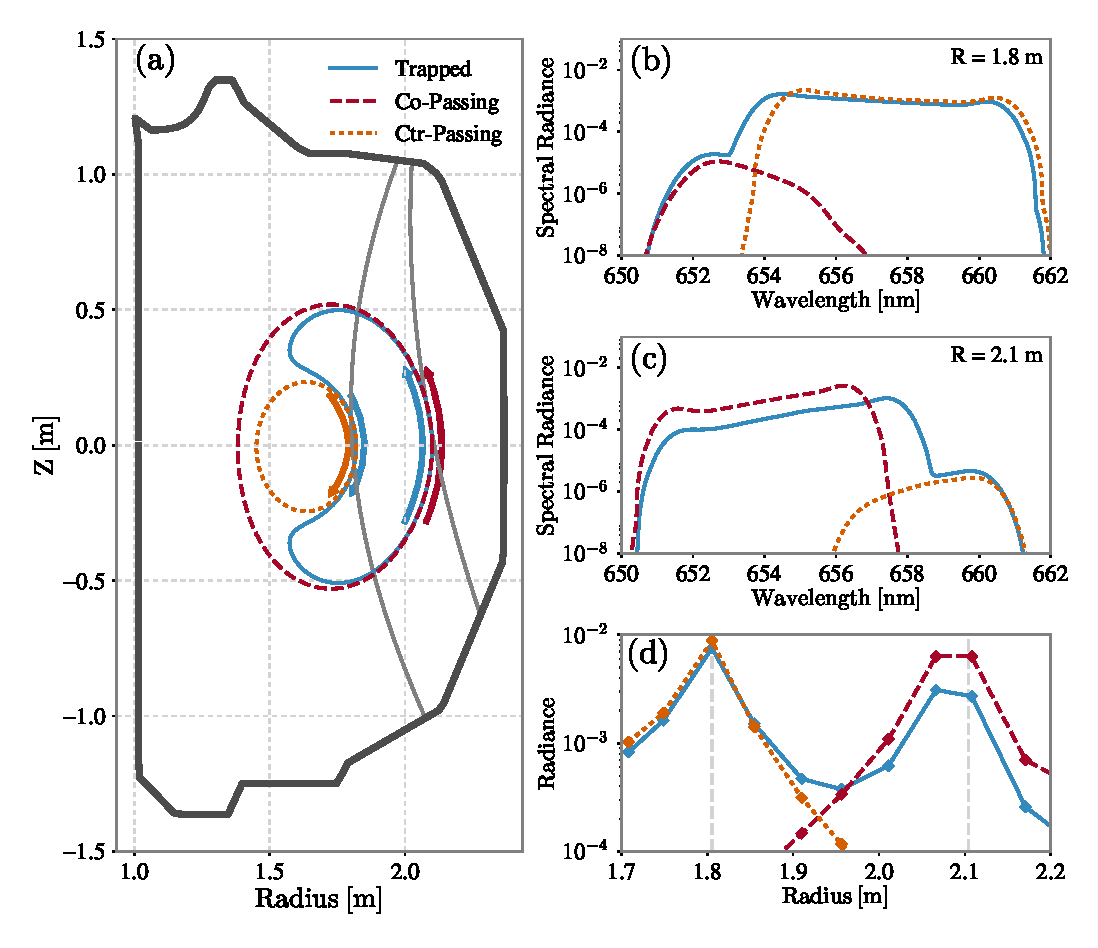
\includegraphics[width=15cm]{figures/orbit_fida_spectra.eps}
    \caption{FIDA orbit weights/spectra produced by three different orbits: trapped ($\rm{\mathbf{J}=(50\;keV,\;0.5,\;2.1\;m)}$), co-passing ($\rm{\mathbf{J}=(50\;keV,\;0.7,\;2.1\;m)}$), and counter passing ($\rm{\mathbf{J}=(50\;keV,\;-0.5,\;1.82\;m)}$). Arrows indicate direction of the fast-ion poloidal velocity. (a): Polodial projection of the orbits and oblique FIDA chords. (b): FIDA spectra produced by the orbits at R=1.8 m. (c): FIDA spectra produced by the orbits at R=2.1 m. (d): Radial profile of FIDA spectra integrated from 647-667 nm.}
    \label{fig:orbit_fida_spectra}
\end{figure}
In Orbit tomography, the fundamental quantity is the fast-ion orbit. This is more natural then the ``pixels'' used in Velocity-space Tomography. Unlike ``pixels'', fast-ion orbits naturally correlate different spatial locations.
Figure \ref{fig:orbit_fida_spectra} shows the wavelength dependent FIDA weight functions for a co-passing, counter-passing, and trapped orbit. Consider the innermost viewing chord in Figure \ref{fig:orbit_fida_spectra}a. The counter-passing and trapped orbits are moving away from the camera, producing strong red-shifted spectra (Fig. \ref{fig:orbit_fida_spectra}b). Interestingly, the co-passing orbit, despite being spatially separated from the collection region of the innermost viewing chord, produces a weak blue-shifted spectrum. The opposite is seen in the outermost viewing chord, Figure \ref{fig:orbit_fida_spectra}c, where the co-passing and trapped orbits produce a strong blue-shifted spectra and the counter-passing orbit produces a weaker red-shifted spectrum. The fast-ion orbits are correlating the different viewing chords together. Figure \ref{fig:orbit_fida_spectra}d proves this assertion by showing the integrated FIDA signal produced by each orbit over a radial array of viewing chords. Since the viewing chords are sensitive, to varying degrees, to all the orbits, any diagnostic, regardless of geometry, can be used in Orbit Tomography. This is a large improvement over Velocity-space Tomography, which is limited to spatially overlapping diagnostics. 

However, the largest advantage Orbit Tomography has over Velocity-space Tomography is the ability to infer the entire fast-ion distribution, not just a local approximation. In Velocity-space Tomography, there is no way to know how different spatial locations are related. In Orbit Tomography, orbits connect different locations together---measuring one part of the orbit automatically gives information along the entire orbit. This allows us to gain information about spatial locations that are not directly measured. Multiple radial FIDA arrays are then sufficient to infer the \textit{entire} fast-ion distribution function. 

In the following sections, we discuss how Orbit Tomography is done in practice. We examine how the irregularly shaped orbit-space necessitates an irregular grid and the development of a new inference method. We then characterize the inference method in the same manner as the velocity-space inference methods discussed in the previous chapter.
We then demonstrate the technique using experimental FIDA data from a classically described DIII-D discharge. Finally, Orbit Tomography is used to study the redistribution of fast ions by a sawtooth crash in an ASDEX Upgrade discharge.

\section{Orbit Tomography Formulation}\label{sec:orbit_tomography}
Orbit Tomography has a few technical details that must be handled with care. In the following subsections, we will examine these details in order to provide a guide to performing Orbit Tomography.

\subsection{The Orbit-space Grid}
The number of orbits used in the linearized forward model (Eq. \ref{eq:Wxn}) dictates its accuracy---the more orbits, the more accurate the model.
However, adding an orbit to the forward model also adds a free parameter to the inverse problem, making it more difficult to solve and more likely to produce solutions with large variances.
Care must be taken when selecting the number of orbits as to balance theses two goals.
This is complicated by the irregular shape of the orbit-space (Fig. \ref{fig:orbit_topology}). The irregular shape makes it difficult to choose orbits that are representative of the orbit space.

A naive approach would be using a regularly spaced Cartesian grid. While conceptually simple, the number of orbits needed to faithfully represent the space would exceed our ability to accurately solve the inverse problem. An irregular grid, however, would be able to faithfully represent the space with fewer orbits.
We can construct an irregular grid by first computing a fine Cartesian grid and then use a clustering algorithm to split the orbits into an arbitrary number of clusters. The centers of the clusters become the coordinates of the orbits used in the analysis. Figure \ref{fig:orbit_cluster}a shows the orbits that reside in a cluster and the central orbit. The number of clusters/orbits used depends on the quality and quantity of the available data. When first clustering the orbits, take care not to cluster orbits of different topologies since they have orbit weights that are discongruent with each other.
\begin{figure}[h!]
    \centering
    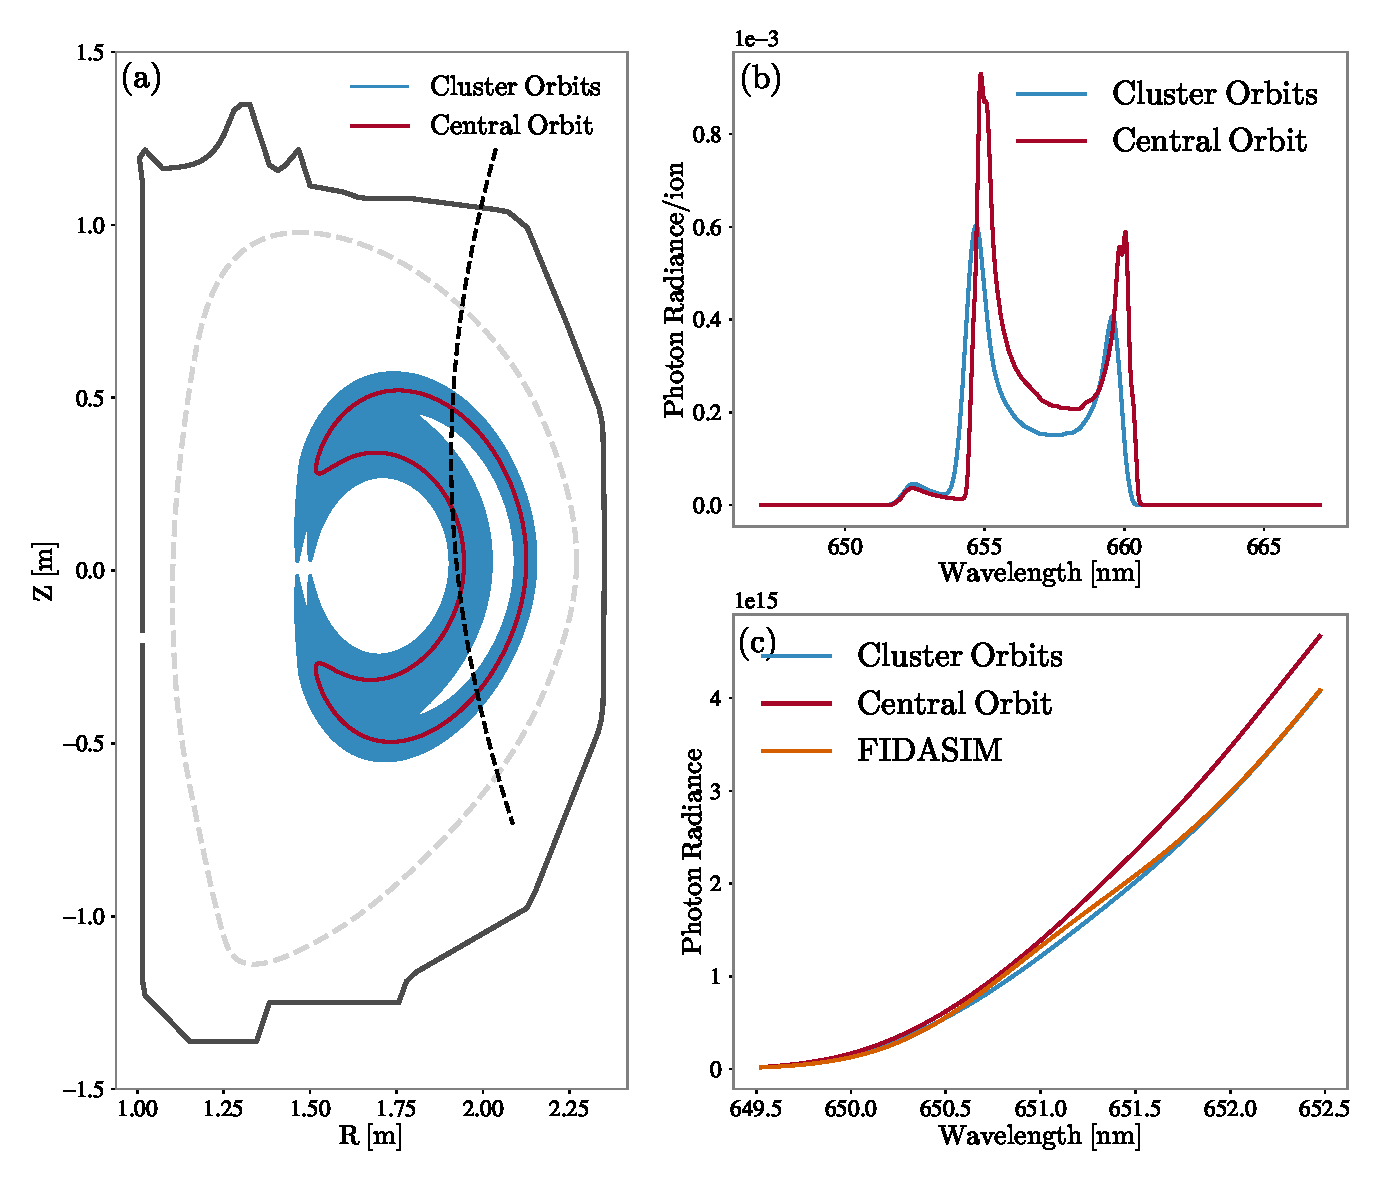
\includegraphics[width=15cm]{figures/orbit_cluster.eps}
    \caption{(a) Poloidal projection of an orbit cluster (blue) and the cluster's central orbit (red). (b) The wavelength dependent orbit weight functions for an oblique line of sight (dashed line). The weight function calculated using only the central orbit is shown in red. The average of the weight functions of the orbits within the cluster is shown in blue. (c) Spectra produced using the different weight functions: single orbit weight function (red), averaged weight function (blue). Spectra calculated by full forward model, FIDASIM, is shown in orange. The averaged weight functions produce spectra closer to the full forward model.}
    \label{fig:orbit_cluster}
\end{figure}

Another consideration is the problem of balancing the resolution of the orbit-space and configuration-space---the space where the diagnostics collects data.
As mentioned in the discussion about including the effects of the radial electric field in Chapter \ref{chap:weights}, the orbit weight functions are sensitive to the locations of the fast-ions relative to the diagnostic's collection region.
The orbits need to faithfully represent \textit{both} orbit-space and configuration-space.
Fortunately, the clustering method naturally allows for increased coverage of configuration-space while also limiting the number of orbits used.
By averaging the orbit weights of the individual orbits within a cluster, instead of only using the weight function of the central orbit, the spatial affects can be partially accounted for---essentially acting like a compromise between a fine and coarse grid. Figure \ref{fig:orbit_cluster}b shows the difference between the central orbit's weight function and the averaged weight function.
The averaging greatly increases the time needed to calculate the orbit weights but also increases the accuracy of the linearized forward model (Fig \ref{fig:orbit_cluster}c), which reduces a source of systematic bias.
It should be mentioned that this process of averaging the orbit weights within each cluster is not strictly necessary and is only recommended if the weight functions of central orbits produce spectra that are significantly different from the full forward model.

\subsection{Bayesian Inference Method}
Since we can control the number of orbits used in the inference, we typically design systems to be under-determined---making the inverse problem easier to solve.
Despite this, naive solutions (Eq. \ref{eq:least_squares_solution}) have non-physical characteristics, such as many sharp gradients and negative values. The solutions are also very sensitive to noise.
As seen in the chapter on Velocity-space Tomography, this is a very common problem and strategies have been developed to regularize these types of systems to be well behaved. Unfortunately, many of the techniques are incompatible with an irregular grid.
Additionally, the regularization techniques are inflexible and unable to incorporate new types of constraints or hyper-parameters. For these reasons, we use a Bayesian technique to infer the distribution.

\subsubsection{Bayesian Background}
Unlike some of the previous studied inversion methods, Bayesian techniques do not seek to find a solution that minimizes a cost function but seeks to determine the \textit{distribution} of solutions that are consistent with both measured data and prior knowledge about the solution.

Bayesian techniques are probabilistic in nature and, as such, deal with manipulating probability distributions. The main tools for doing this is Bayes rule,
\begin{equation}\label{eq:bayes_rule}
    \rm{prob}(X|\,Y) = \frac{\rm{prob}(Y|\,X) \times \rm{prob}(X)}{\rm{prob}(Y)}\,,
\end{equation}
and marginalization,
\begin{equation}\label{eq:marginalization}
    \rm{prob}(X) = \int_{-\infty}^{\infty} \rm{prob}(X,Y)\,dY .
\end{equation}
Bayes rule provides a rigorous framework for incorporating prior information and marginalization provides a method of dealing with nuisance parameters---parameters that are needed in the forward model but are not of interest.

Bayes rule consists of 4 distinct terms.
The $\rm{prob}(X)$ term is called the prior probability and it encodes prior knowledge about the model parameter, $X$.
The next term, $\rm{prob}(Y|\,X)$, is called the likelihood probability and is the probability of the data, $Y$, given the model parameter, $X$---the symbol $(|)$ denotes a conditional relationship and should be read as ``given''.
The likelihood probability is where measurement error can be accounted for, usually in the form of a Gaussian distribution.
Multiplying the likelihood probability with the prior probability can be thought of as updating our prior knowledge about the model parameters to be consistent with measurements.
The term, $\rm{prob}(Y)$ (sometimes denoted as $\mathcal{Z}$), is called the evidence or marginal likelihood and it is the probability of our data occurring under the assumed model.
As will be seen later, the evidence is useful for model selection and choosing hyper-parameter values. For parameter estimation problems, the evidence acts as little more than a normalization constant and can be ignored. 
The final term, $\rm{prob}(X|\,Y)$, is called the posterior and it is the probability of the model parameters, $X$, given the data, $Y$. It represents the updated knowledge about the model parameters after incorporating the knowledge learned from the measurements.
Once the posterior is known, the best set of parameters is found by either computing the mean value of the parameters or, when calculating the mean is intractable, by finding the parameters that maximize the posterior, the maximum a posteriori (MAP) estimate.

\subsubsection{Prior \& Likelihood Probabilities}
There are several pieces of prior information that can be exploited.
First off, though it may not be immediately obvious, there is strong prior information in the well-diagnosed magnetic equilibrium.
Whatever form the estimate of the fast-ion distribution function takes, the magnetic equilibrium must be able to support it---just as an architect can only redesign a house to be consistent with its existing framing.
Fortunately, this \textit{structural} constraint is already incorporated in the form of the trajectories of the fast-ion orbits, ensuring that our estimate of the distribution function will, at least, be consistent with the magnetic equilibrium.  
The rest of our prior information is rather obvious: the distribution should be smooth, non-negative, and ``close'' to  theoretical predictions. The smoothness and ``closeness'' can be represented by using a Gaussian Process prior:
\begin{equation}\label{eq:prior}
    \rm{prob}(\mathbf{n}|\boldsymbol{\mu_n},\boldsymbol{\theta},\{\mathbf{J}\})  =
    \mathcal{N}(\boldsymbol{\mu_n},\mathbf{\Sigma_n(\boldsymbol{\theta},\{\mathbf{J}\}}))\,,
\end{equation}
where $\mathbf{\Sigma_n(\boldsymbol{\theta},\{\mathbf{J}\}})$ is a covariance matrix---or kernel in Gaussian process parlance---that correlates the different orbits, $\{\mathbf{J}\}$, according to the hyper-parameters, $\boldsymbol{\theta}$. $\boldsymbol{\mu_n}$ is a guess distribution---usually the theoretical prediction, but, if the data are good enough, an all zero null distribution would suffice.
The best choice of the form of the covariance matrix is still an open question, but here a standard squared exponential kernel in orbit-space is used, 
\begin{equation}\label{eq:kernel}
    {\Sigma_n}_{ij} = \theta_1^2 \exp \left (-\frac{1}{2\theta_2^2}\left ( (\mathbf{J}_i - \mathbf{J}_j)^T\cdot (\mathbf{J}_i - \mathbf{J}_j)\right ) \right ) \;.
\end{equation}

The experimental data, $\mathbf{d}$, is normally distributed around the linearized forward model's prediction, yielding the following for the likelihood probability,
\begin{equation}\label{eq:likelihood}
    \rm{prob}(\mathbf{d}|\mathbf{n},\boldsymbol{\theta},\{\mathbf{J}\}) = \mathcal{N}(\mathbf{W}\cdot\mathbf{n},\mathbf{\Sigma_d}) \,,
\end{equation}
where $\mathbf{\Sigma_d}$ is a diagonal matrix whose diagonal elements contain the variances/errors of the measurements.

\subsubsection{Posterior and Hyper-parameter Selection}
With the prior and the likelihood specified, we can then define the posterior to be
\begin{equation}\label{eq:posterior}
    \rm{prob}(\mathbf{n}| \mathbf{d}, \boldsymbol{\theta}, \{\mathbf{J}\}) = \mathcal{Z}^{-1} \mathcal{N}( \boldsymbol{\mu}, \mathbf{\Sigma})\,,
\end{equation}
where
\begin{equation}
    \mathbf{\Sigma} = (\mathbf{W}^T \cdot \mathbf{\Sigma_d}^{-1} \cdot \mathbf{W} + \mathbf{\Sigma_n}^{-1})^{-1} \;  
\end{equation}
and
\begin{equation}
    \boldsymbol{\mu} = \mathbf{\Sigma}\cdot\mathbf{W}^T\cdot\mathbf{\Sigma_d}^{-1} \cdot \mathbf{d} + \mathbf{\Sigma} \cdot \mathbf{\Sigma_n}^{-1} \cdot \boldsymbol{\mu_n}\;
\end{equation}
are the posterior covariance and mean, respectively.
The last piece of prior information we have is that the distribution should be positive; however, since the posterior takes the form of a multivariate normal distribution, positivity of the mean, $\boldsymbol{\mu}$, is not guaranteed.
To enforce non-negativity, an optimization algorithm is used to maximize the posterior subject to a positivity constraint.

The hyper-parameters in the prior (Eq. \ref{eq:prior}), $\boldsymbol{\theta}$, are chosen via log-evidence maximization. The process of maximizing the log-evidence is equivalent to calculating Bayes factors used in model comparison problems.
Ignoring terms that do not depend on the hyper-parameters, the log-evidence is given by
\begin{equation}
\begin{aligned}\label{eq:log_evidence}
    \log{\mathcal{Z}} = \frac{1}{2} &(-\log(|\mathbf{\Sigma_n}^{-1}|) -\log(|\mathbf{\Sigma}^{-1}|)\,- \\
    & (\mathbf{d} - \mathbf{W} \cdot \boldsymbol{\mu})^T \cdot \mathbf{\Sigma_d}^{-1} \cdot (\mathbf{d} - \mathbf{W}\cdot\boldsymbol{\mu})\,- \\
    & (\boldsymbol{\mu} - \boldsymbol{\mu_n})^T \cdot \mathbf{\Sigma_n}^{-1} \cdot (\boldsymbol{\mu} - \boldsymbol{\mu_n}) )\;. 
\end{aligned}
\end{equation}
The log-evidence is maximized using standard optimization algorithms.

\section{Benchmark using Synthetic Data}
The above inference method is benchmarked using synthetic data generated from the linearized forward model (Eq. \ref{eq:Wxn}) using a known distribution function. 
The benchmark case is modeled after DIII-D shot \#171469; a MHD-quiescent plasma with a fast-ion distribution function that is well described by theoretical models(Fig. \ref{fig:171469_distribution}a).
\begin{figure}[h!]
    \centering
    \includegraphics[width=16cm]{figures/171469_distribution.eps}
    \caption{(a): Theoretical fast-ion distribution function in orbit-space for the MHD-quiescent H-mode of DIII-D discharge \#171469. (b): The theoretical distribution function down-sampled onto the clustered 1000-orbit grid. The mapping is done as follows: the fast-ions in the theoretical distribution are assigned to the nearest cluster center. The number of fast ions in each cluster is then spread out among the cluster's orbits.}
    \label{fig:171469_distribution}
\end{figure}
The orbit-space is clustered into 1000 representative orbits. The theoretical fast-ion distribution function is down-sampled onto this orbit grid (Fig. \ref{fig:171469_distribution}b). Since the synthetic data is being generated from Equation \ref{eq:Wxn}, the accuracy relative to the full forward model is not relevant and, as such, the central orbits's weight functions are used as they are faster to calculate. 

In addition to the standard FIDA systems used during most shots, the diagnostics used in shot \#171469 were in the so called ``All out FIDA'' configuration, which had most of the available spectroscopic diagnostics tuned to view the FIDA wavelength region.
This diagnostics configuration was used to maximize the number of measurements that are used to reconstruct the fast-ion distribution function.
Figure \ref{fig:d3d_chords} shows all the FIDA lines-of-sight used in the benchmark.
\begin{figure}[h!]
    \centering
    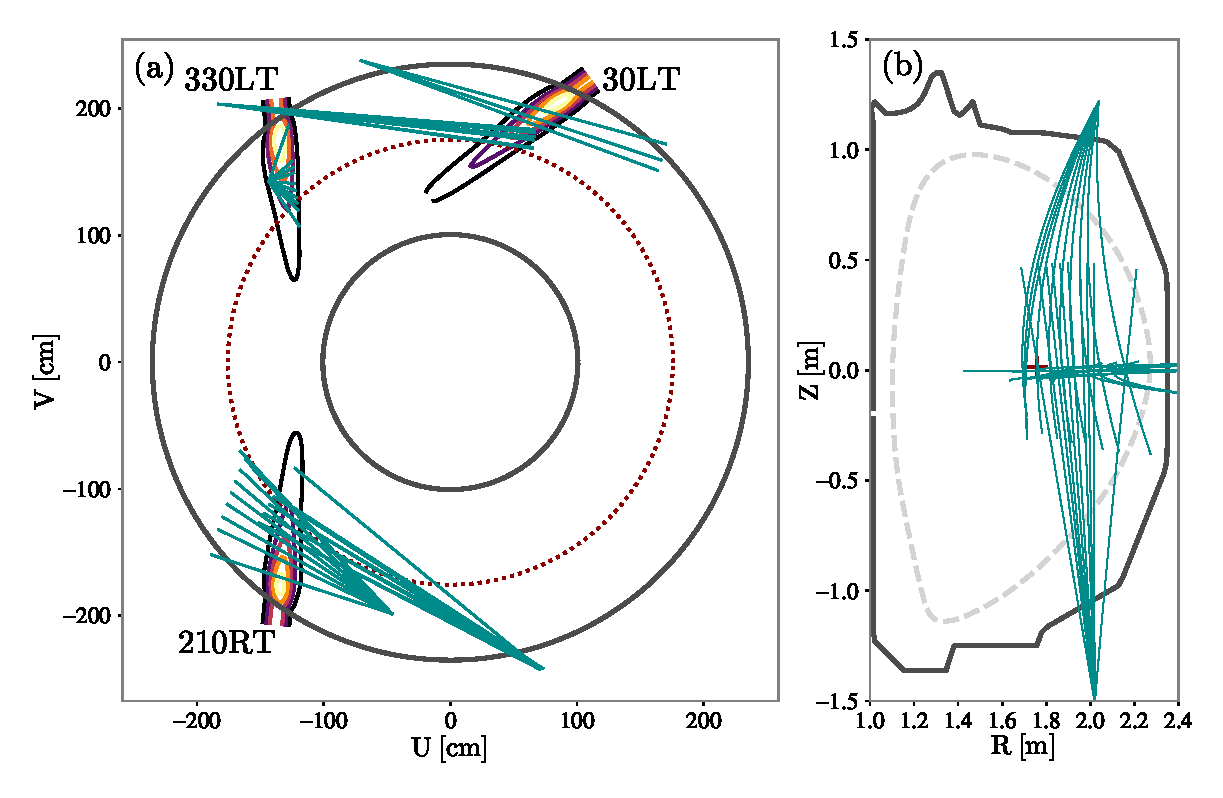
\includegraphics[width=16cm]{figures/d3d_chords.eps}
    \caption{``All out FIDA'' diagnostic setup. 37 FIDA lines-of-sight that view the 210RT, 330LT, and 30LT neutral beams were used.}
    \label{fig:d3d_chords}
\end{figure}
\begin{figure}[h!]
    \centering
    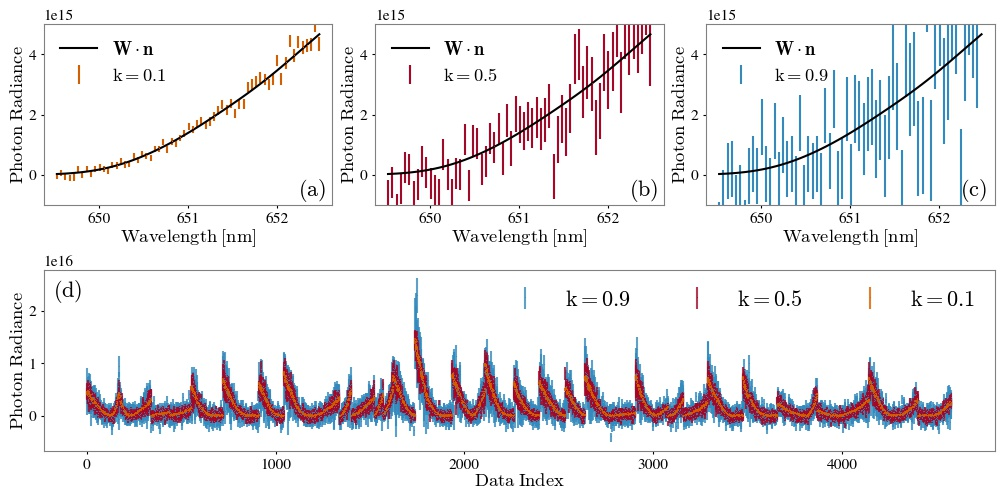
\includegraphics[width=16cm]{figures/synthetic_data.jpg}
    \caption{Synthetic data generated using Equation \ref{eq:Wxn} using the fast-ion distribution in Figure \ref{fig:171469_distribution}b. (a): low noise (k=0.1). (b): medium noise (k=0.5). (c): high noise (k=0.9). (d): The synthetic data vectors for k=0.1 (orange), k=0.5 (red), and k=0.9 (blue). A total of 4579 measurements are used in the benchmark.}
    \label{fig:synthetic_data}
\end{figure}
In experiment, the measured spectra is corrupted by other light sources, limiting the number of available measurements.
For authenticity, the synthetic spectra is similarly limited. The noise model (Eq. \ref{eq:S_noisy}) from Chapter \ref{chap:velocity-space_tomography} is used to add noise to the synthetic spectra. Figure \ref{fig:synthetic_data} shows a sample of the synthetic spectra used in the benchmark for three different noise levels. Since the forward model is exact, the theoretical distribution is not used in the prior as it would have too much of an influence and defeat the purpose of the benchmark---if the prior is perfect why bother with the posterior? A null distribution comprised of all zeros was used.

Figures \ref{fig:synthetic_reconstructions}-\ref{fig:bias_variance_mse} shows the results of the benchmark. Figure \ref{fig:synthetic_reconstructions} show the mean distribution, $\mathbf{n}_\mu$ for three different error levels. All three reconstructions capture the bulk features of the true distribution (Fig. \ref{fig:171469_distribution}b); however, the reconstructions have difficultly capturing fine detail, enhancing the smoothing already present due to the down-sampling. As the error level increases, so does the smoothing. 
\begin{figure}[h!]
    \centering
    \includegraphics[width=16cm]{figures/distribution_error_scan.eps}
    \caption{Reconstructions of synthetic data at 3 different noise levels. Top: low noise (k=0.1). Middle: medium noise (k=0.5). Bottom: high noise (k=0.9). Each distribution is on the same color scale.}
    \label{fig:synthetic_reconstructions}
\end{figure}

Figure \ref{fig:bias_variance_mse} characterizes the variance, bias, and mean squared error (MSE) of the reconstruction for the medium noise case (k=0.5). The top row shows the square root of the variance of the reconstruction, which shows that variance is larger for lower energy ($<25$ keV) fast ions. This makes sense as low energy fast-ions are more likely to produce spectra with small Doppler shift, which would have been corrupted by the thermal halo emission and excluded from the analysis. Since there is little data constraining the reconstruction in those areas, the values of the distribution can vary wildly depending on the data, hence, the larger variance.
\begin{figure}[h!]
    \centering
    \includegraphics[width=16cm]{figures/bias_variance_mse.eps}
    \caption{Variance, Bias, and MSE for the medium noise case (k=0.5). Top row: square root of the variance. Middle row: Bias of the reconstruction. Bottom row: square root of the MSE.}
    \label{fig:bias_variance_mse}
\end{figure}
The middle row shows the bias, $\mathbf{n}_\mu - \mathbf{n}_{\rm{true}}$, of the reconstruction. With the exception of the peak at 20 keV, the bias has similar levels to the $\sqrt{\rm{variance}}$, which occurs when the bias-variance tradeoff is optimized. This indicates that the optimal solution was found. The bottom row shows the square root of the MSE. The MSE is dominated by the peaks in the bias. Otherwise, the MSE is well balanced between the bias and the variance.

\begin{figure}[h!]
    \centering
    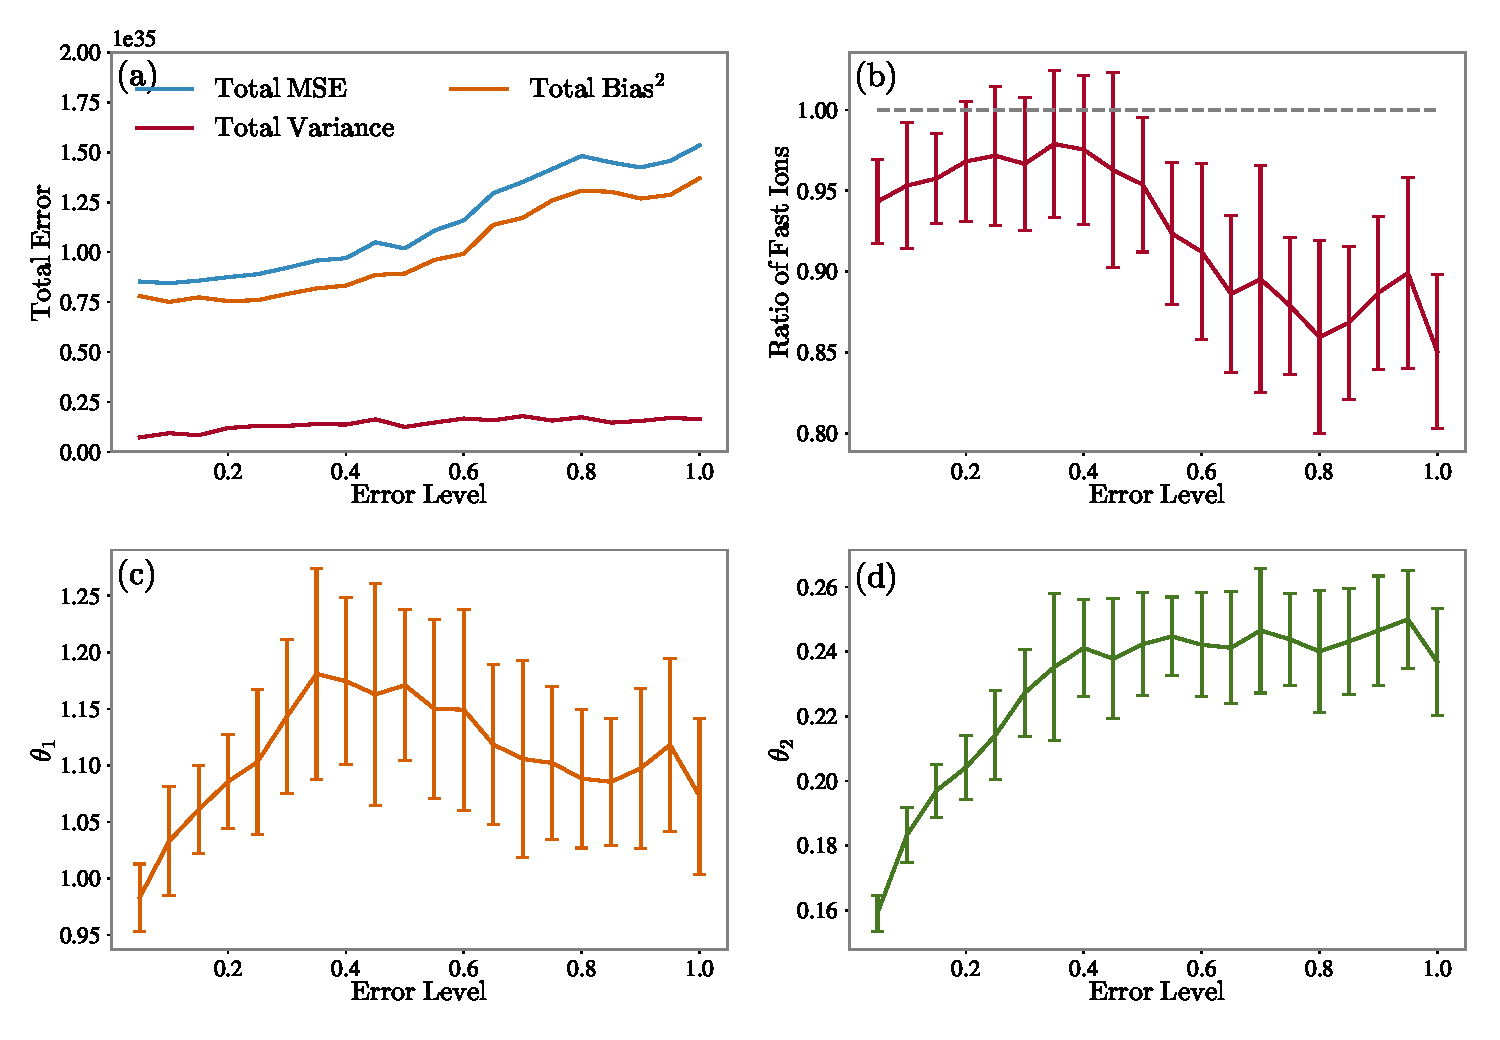
\includegraphics[width=14cm]{figures/error_scan.eps}
    \caption{Error scan of several quantitative metrics. (a): Error scan of the total MSE. (b): Error scan of the ratio of the number of fast ions. A value of one (dashed line) is ideal. (c-d): Error scans of the hyper-parameters.}
    \label{fig:error_scan}
\end{figure}
Figure \ref{fig:error_scan}a shows the total MSE as a function of error level. As the error level increases, so does the MSE. Between the variance and the bias, the bias is the most affected by the increase in noise, remaining steady until an error level of 0.4 and then increasing. Figure \ref{fig:error_scan}b shows the ratio of the number of fast-ions between the true and reconstructed distribution. Throughout the error scan, the ratio is close to one. However, in the beginning of the scan the ratio slightly increases towards the ideal ratio of one until an error level of 0.4 at which the ratio begins to decrease. Figures \ref{fig:error_scan}c-d show the values of the hyper-parameters. The first hyper-parameter, $\theta_1$, controls how far away the distribution can be from the provided mean.  Like the ratio of the number of fast ions, the first hyper-parameter increases until an error level of 0.4 at which it decreases. Since the provided mean was a null distribution, the decreasing value indicates a trend towards the null distribution. This is supported by the decrease in the ratio of the number fast ions after an error level 0.4. The second hyper-parameter, $\theta_2$, controls the amount of correlation between the orbits, i.e. smoothing. As the error increases, so does the amount of smoothing until a error level of 0.4 at which the hyper-parameter no longer changes.

In summary, the inference method has a tendency to produce overly smooth distributions. This tendency increases with error. Additionally, compared to velocity-space tomography, the method is relatively insensitive to increases in noise. This is seen by comparing the rate of increase in MSE in Figure \ref{fig:Qfigs_tomos} and Figure \ref{fig:error_scan}.  

\section{Experimental Reconstructions}\label{sec:experiment}
\subsection{Data Considerations}
The benchmark with synthetic data showed that inference of the full fast-ion distribution function is technically feasible; however, real experimental data can introduce a number of problems.
One issue is that the reconstructions closely resemble the weight functions.
This occurs when the diagnostics have poor coverage of the fast-ion phase-space.
In other words, the weight functions do not overlap, which is an important requirement for all tomography problems.
The whole point of tomographic techniques is to combine the partial information of a parameter contained within multiple measurements to infer the entire parameter. 
If the weight functions do not overlap, the measurements are essentially independent and the information contained within cannot be combined. This leads to learned parameters that are scalar multiples of the weight functions. However, when the weight functions overlap the values the parameters can take are constrained as the value has to agree with multiple measurements, not just one. The more measurements viewing the same region, the more accurate the learned parameter. 
Unfortunately, the only way to resolve this issue is to add weight functions that overlap with the existing weight functions, which is not always possible.

As shown in the benchmark case, a low signal to noise ratio can cause issues. 
If the data are too noisy, many different proposal distributions would be consistent with the data, causing high uncertainty and, possibly, a mean that is far away from the true distribution.
Fortunately, poor signal to noise can be mitigated. If it is assumed that the distribution function does not change over a time period, the experimental data can be averaged over many time slices, increasing the signal to noise. The resulting distribution would also be an average; however, depending on the validity of the steady-state assumption, this may be close to the instantaneous distribution.
Lastly, systematic errors can cause significant problems.
Systematic error usually come in two forms: calibration errors and incomplete models.

In order to do Orbit Tomography the diagnostics must be absolutely calibrated, especially if multiple diagnostics are used.
Consider two diagnostics viewing the same region of phase-space, call them A and B.
The distribution function that produced the data for diagnostic A is the same distribution that produced the data for diagnostic B.
During the reconstruction, they would both agree on the distribution that produced their respective data.
However, if diagnostic B was unknowingly miscalibrated, the diagnostics would be in disagreement.
In order to ensure consensus among the diagnostics, special care must be taken to guarantee the calibration factors are correct.
In some cases, the absolute calibration of a diagnostic can drift during the course of an experimental campaign.
In these cases, the calibrations can be corrected for by using a reference discharge. In a reference discharge the experimental conditions are well described by theoretical models and the experimental data should agree with the forward models of the diagnostics. Any drift in the absolute calibration can then be corrected for by scaling the data to match the output of the forward models. The calculated scale factors are then used to correct the data of subsequent discharges.

Systematic error introduced by incomplete models is harder to deal with.
If a measurement is a mixture of signal produced by the fast-ion distribution function and signal produced by another unknown source, the forward model, unaware of the second source, will wrongly assume that all of the signal comes from the fast-ion distribution function. In the best case scenario, the second source is constant across measurements. In this case, the inferred distribution would have a constant bias. However, if the corrupting source is different for each measurement, it would wreak havoc on the reconstruction, as none of the measurements would be consistent with each other. It would be like every measurement was miscalibrated by a different scale factor.  
The only way to fix this is by including the second source into the forward model.

It cannot be stated more strongly: all efforts should be undertaken to eliminate sources of systematic error.
However, if this is not possible, the effects of systematic error, as well as random noise, can be reduced by limiting the number of free parameters used in the reconstruction.
By reducing the number of free parameters, the model becomes less flexible, making it harder for the distribution function to contort itself trying to fit all the error ridden data.
In other words, it makes it easier for the diagnostics to compromise on a solution that captures the broad strokes of the distribution, if not the fine details. 

\subsection{Reconstruction of a Classical Fast-ion Distribution}
Keeping in mind the possible issues that can arise when attempting Orbit Tomography with real data, here we reconstruct the fast-ion distribution from the discharge that our benchmark case is based on, the MHD-quiescent, DIII-D discharge \#171469. While previous benchmark demonstrated that Orbit Tomography is technically feasible in an idealized scenario, here we demonstrate that Orbit Tomography is possible in experimental conditions.

\begin{figure}[h!]
    \centering
    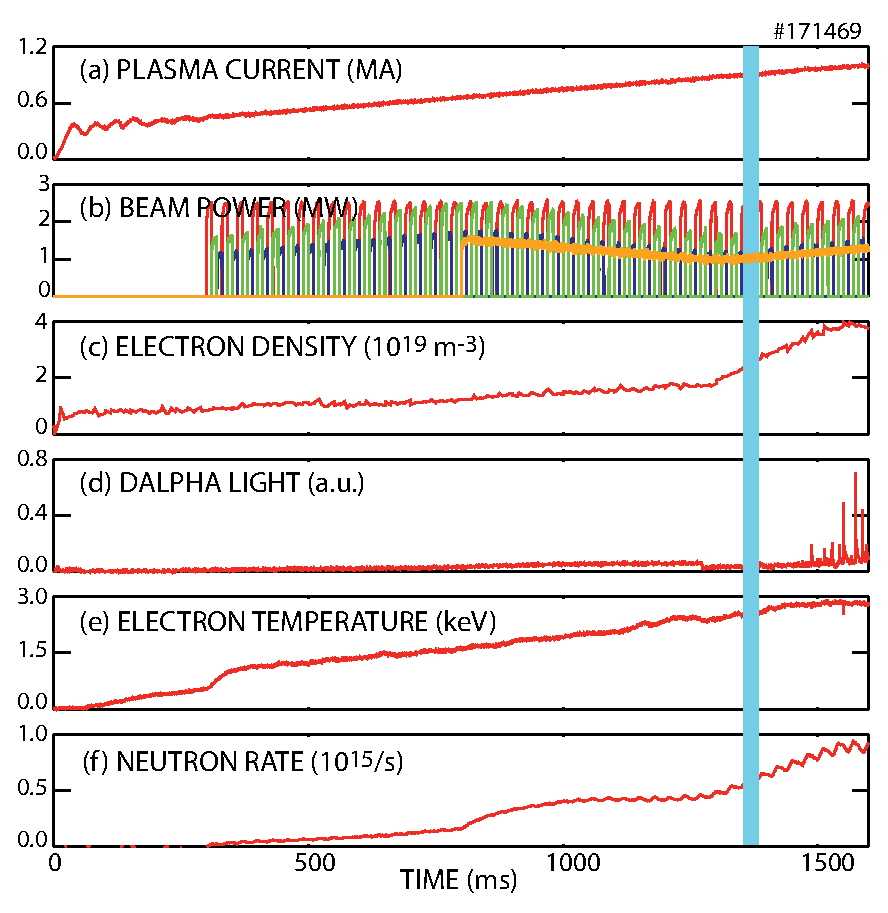
\includegraphics[width=16cm]{figures/171469_plasma.eps}
    \caption{Time evolution of (a) plasma current, (b) beam power of the four utilized sources, (c) line-average electron density, (d) D$_\alpha$ light from the lower divertor, (e) central electron temperature as measured by ECE, and (f) volume-average neutron rate. The vertical line indicates the selected analysis time.}
    \label{fig:d3d_plasma}
\end{figure}
The discharge conditions for the measurements appear in Figure \ref{fig:d3d_plasma}. At the selected analysis time, the plasma current is $I_p=0.91$~MA (Fig. \ref{fig:d3d_plasma}a). Four different neutral-beam sources inject an average neutral-beam power of 2.7~MW (Fig.\ref{fig:d3d_plasma}b). All of the sources inject near-tangentially in the midplane (tangency radius $R_{tan}=115$~cm). To facilitate time-slice subtraction, three of the sources act as active FIDA beams and are only on one-third of the time. In this discharge, the new capability to vary the injection energy during the discharge \cite{pace2016control} was employed on three of the four sources; the selected analysis time is near a minimum of beam voltage and power (Fig. \ref{fig:d3d_plasma}b). At this time, one 81.5~keV co-current source injects an average power of 0.8~MW, two 64.7~keV co-current sources inject an average power of 1.5~MW, and one 65.6~keV counter-current source injects an average power of 0.4~MW. The toroidal field of 1.9~T is in the clockwise direction, which implies downward $\nabla B$ and curvature drifts. The plasma configuration is an elongated ($\kappa\simeq1.8$), lower single null configuration with upper and lower triangularity of $\delta=0.35$ and 0.6, respectively. In this configuration, the power threshold for the L-to-H transition is relatively low, so an H-mode is triggered at 1272~ms and causes rising electron density (Fig. \ref{fig:d3d_plasma}c) and a sudden drop in cold D$_\alpha$ light from recycling deuterium atoms (Fig. \ref{fig:d3d_plasma}d).  To avoid ELM contamination of the FIDA signals, the selected analysis time is from 1350-1380~ms, shortly before the first ELM at 1385~ms.  The central electron temperature is 2.5~keV at this time (Fig. \ref{fig:d3d_plasma}1e) and the neutron rate is $2.9\times10^{14}$~sec$^{-1}$ (Fig. \ref{fig:d3d_plasma}f).
No significant MHD occurs at the chosen time of interest. By 1400~ms, a $\sim70$~kHz mode is observed on the magnetics and on the cross-power of two CO$_2$ interferometer chords, but this mode is undetectable between 1350-1380~ms.

The same reconstruction setup as the benchmark case is used with two exceptions: the weight functions are averaged over the orbits within each cluster and the theoretical prediction is used in the prior. 
Figure \ref{fig:d3d_data} shows the experimental data used in the reconstruction compared against the theoretical prediction. Unlike the benchmark case, the noise level varies across the different lines-of-sight. The mean error level is about k=0.3. Additionally, the three different neutral beams that the lines-of-sight view can interfere with each other. To prevent this affecting the data, the three beams were cycled on and off: 210RT$\rightarrow$30LT$\rightarrow$330LT. This sequence was chosen so that only one beam is on at a time and subsequent beam in the cycle does not corrupt the preceding beam, providing a window to collect background signal for time-slice subtraction. As a result, the data are collected over a range of 30 ms, 10 ms for each beam. It is assumed that the fast-ion distribution does not change appreciably in this time window. Apart from a few lines-of-sight that are underestimated by the theoretical prediction, the experimental data agree with the theoretical prediction.
\begin{figure}[h!]
    \centering
    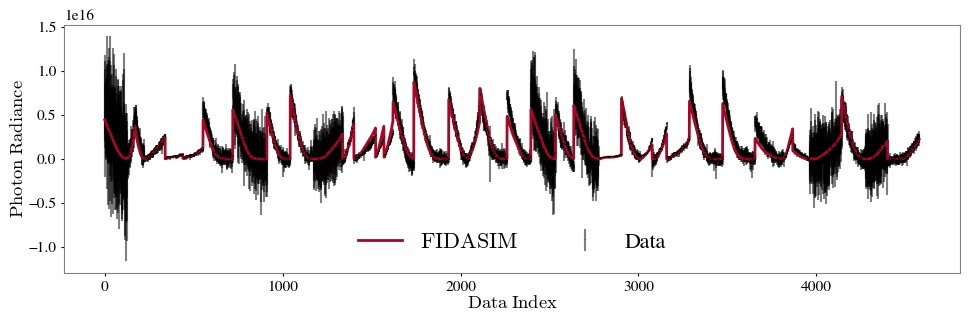
\includegraphics[width=16cm]{figures/d3d_data.jpg}
    \caption{Theoretical (blue line) and Experimental (black lines) FIDA signal for DIII-D shot \#171469. With an exception of the few lines-of-sight that have more signal than expected, the theoretical signal agrees with experiment.}
    \label{fig:d3d_data}
\end{figure}

\begin{figure}[h!]
    \centering
    \includegraphics[width=16cm]{figures/171469_reconstruction.eps}
    \caption{Theoretical (a) and reconstructed (b) fast-ion distribution.for DIII-D shot \#171469. Both distributions are on the same color scale. The reconstructed distribution over-estimates the total number of fast-ions by 37\%.}
    \label{fig:d3d_reconstruction}
\end{figure}
Figure \ref{fig:d3d_reconstruction} shows both the theoretical and reconstructed fast-ion distribution functions. Comparing the two distributions shows that the reconstruction over-estimates the number of fast ions, especially in the lower energy regions. Given that a few of the lines-of-sight had more signal than predicted, this is not surprising. The ratio of the number of fast ions is 1.37, which is larger than what was suggested by the synthetic data benchmark. This indicates that our reconstruction, despite our best efforts, suffers from a systematic error, either from an unknown light source or a calibration error. Given that many of the lines-of-sight were co-opted from other systems that do not typically view D-$\alpha$ emission, the likely source of the systematic error is miscalibration. It could also be that our ``well-understood'' distribution is not so well understood. However, despite the aforementioned problems, the reconstruction is similar to the theoretical prediction verifying that Orbit Tomography is possible in experimental conditions. 

\subsection{Redistribution of Fast Ions by a Sawtooth Crash}
As seen in the previous section, the effects of systematic errors and biases can hamper Orbit Tomography. However, this does not diminish its usefulness in the study of relative changes in the fast-ion distribution function. As mentioned in the previous chapter, while a reconstruction may suffer from systematic error or biases, the errors are stationary. The classic example is a miscalibration, which does not change over many discharges. The reconstructed distributions may be a bit off, but they are consistently off, making the study of relative changes in the distribution possible. We, therefore, take a page from the previous chapter and study the relative changes in the fast-ion distribution induced by a sawtooth crash.

As stated in the previous chapter, a sawtooth instability occurs when the central safety factor, $q_0$, drops below one. When this occurs a $n=m=1$ internal kink can form and grow unstable, causing a magnetic reconnection event, i.e. crash. During the crash, the magnetic fields within the $q=1$ surface changes, perturbing the fast-ion population. From previous publications and the previous chapter, it is known that there is a reduction in the number of fast ions within the $q=1$ surface\cite{jacobsen_stagner2016,van2010imaging,weiland2016}. Other publications also indicate that there is a corresponding increase in the number of fast ions outside the $q=1$ surface.\cite{weiland2016,du2018inpa} This can be seen in Figure \ref{fig:inpa_sawtooth}\cite{du2018inpa} which shows the percent change in the Imaging NPA image, clearly showing both the decrease and increase in the fast-ion density inside and outside of the $q=1$ surface.
Additionally, it is known from the previous chapter and other publications\cite{Muscatello2012,jacobsen_stagner2016,weiland2016} that the sawtooth crash primarily affects the passing fast ions in the core since they are more closely tied to flux surfaces. This is seen in a pronounced reduction in fast-ion density where the pitch is greater than 0.5.
\begin{figure}[h!]
    \centering
    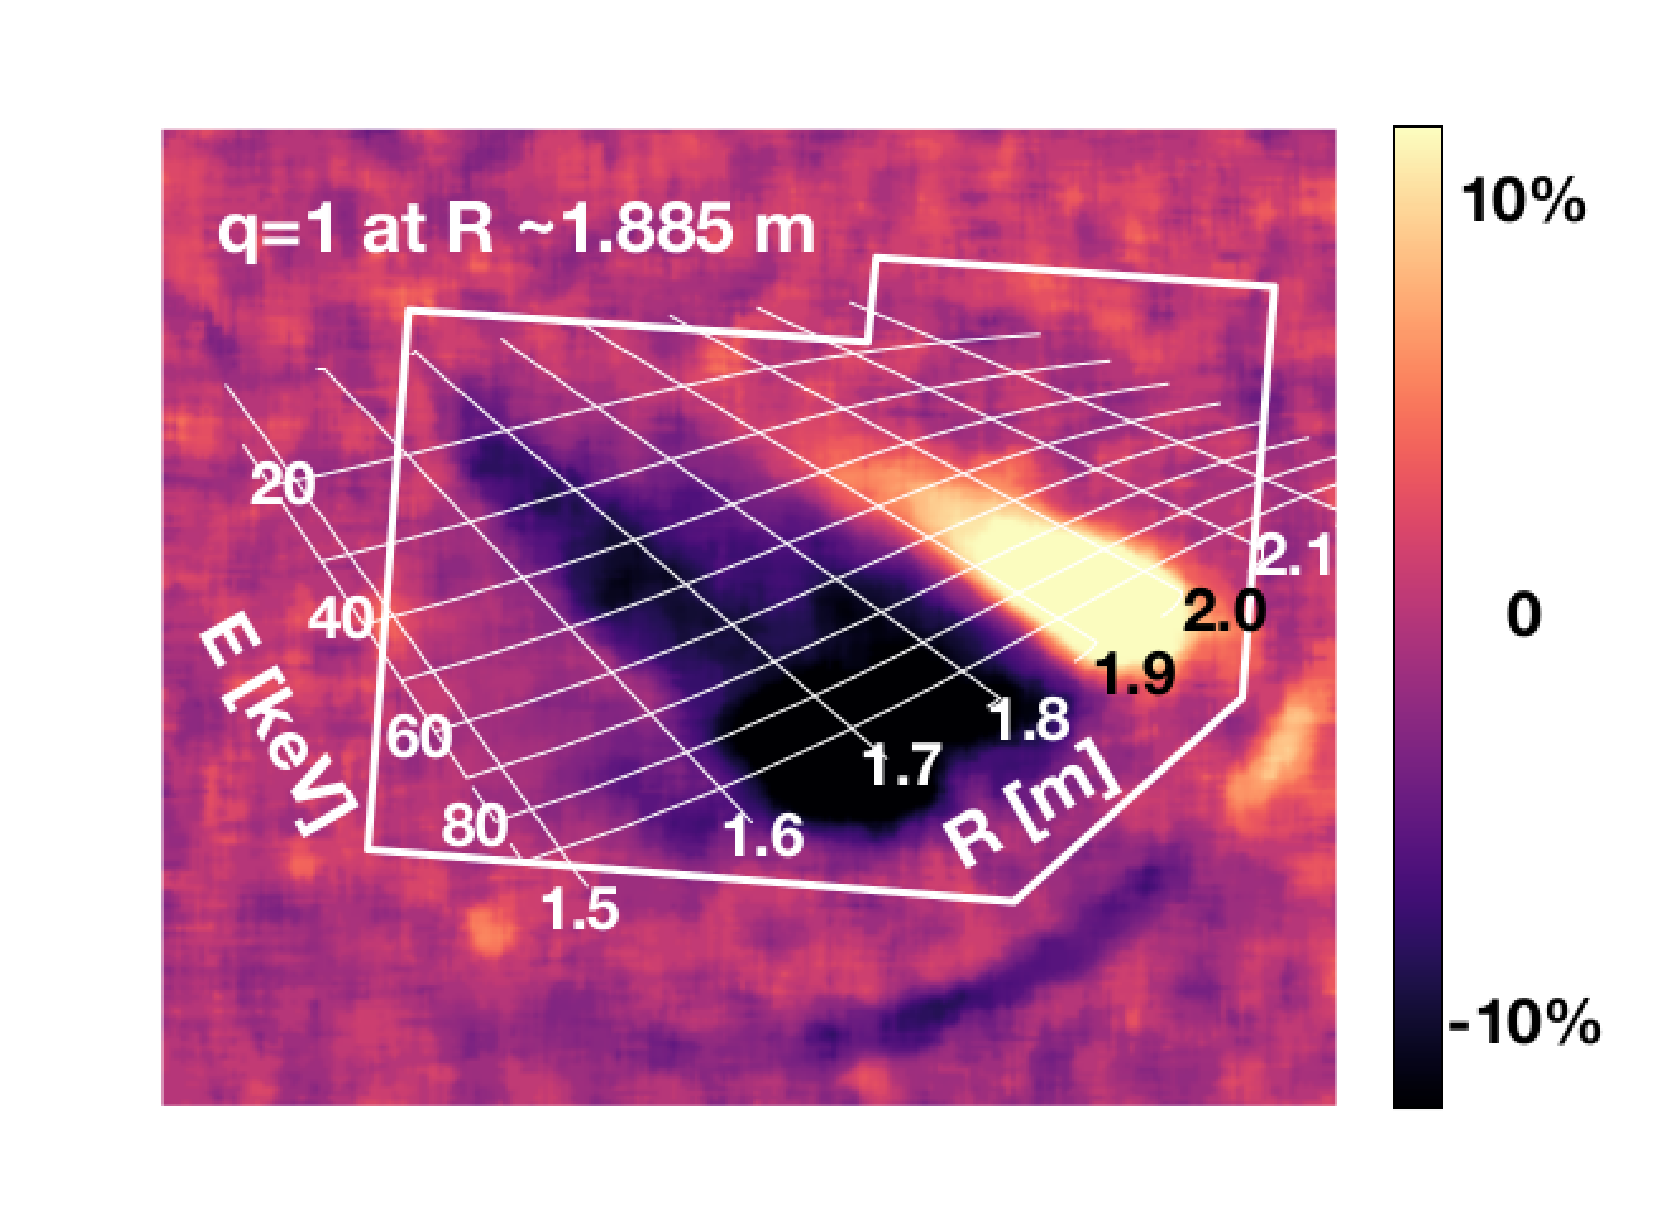
\includegraphics[width=10cm]{figures/inpa_sawtooth.eps}
    \caption{Relative change in the INPA image caused by a sawtooth crash. Within the $q=1$ surface at 1.885 m the signal decreases, while outside the $q=1$ surface the signal increases. Figure courtesy of Xiaodi Du\cite{du2018inpa}}
    \label{fig:inpa_sawtooth}
\end{figure}

\begin{figure}[h!]
    \centering
    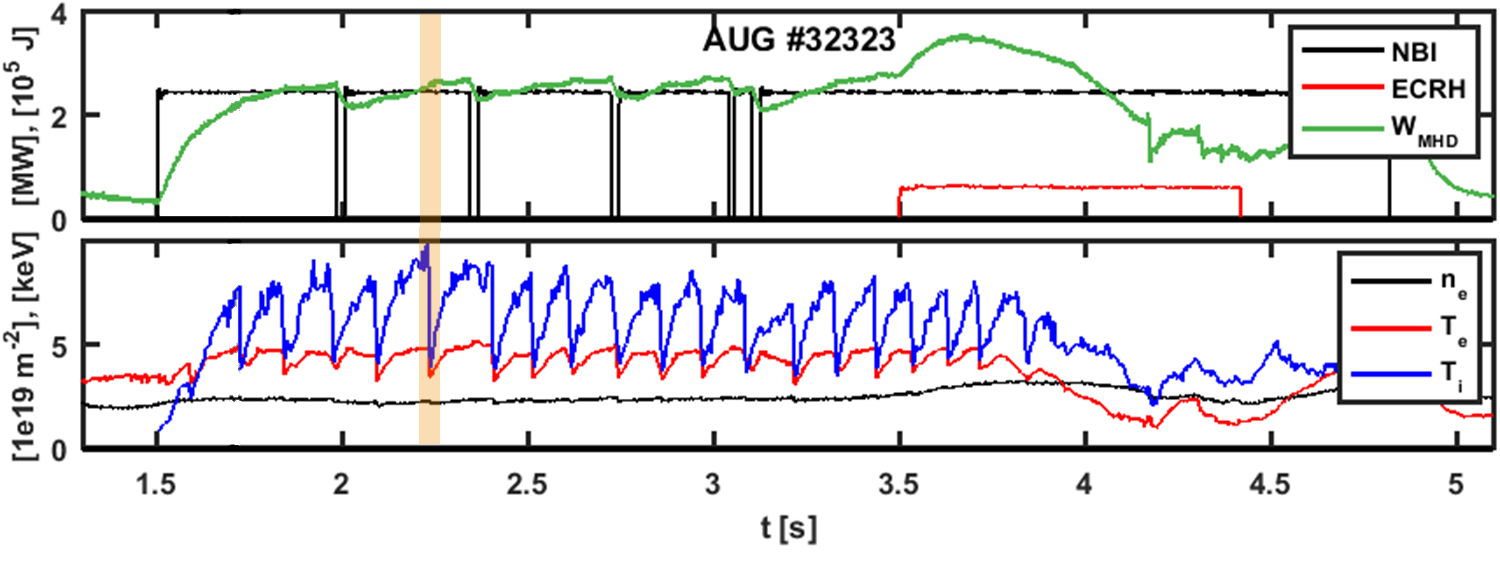
\includegraphics[width=16cm]{figures/32323_plasma.png}
    \caption{Time evolution of the ASDEX Upgrade shot \#32323. Top: auxiliary heating provided by neutral beam injection and ECRH and plasma stored energy W$_{\rm{MHD}}$. Bottom: line-averaged electron density and the ion and electron temperatures in the plasma center. The time of interest is highlighted in orange: 2.236 s. Figure courtesy of Mirko Salewski.\cite{salewski2018deuterium}}
    \label{fig:augd_plasma}
\end{figure}
For our analysis we use ASDEX Upgrade shot \#32323, which was previously studied with Velocity-space Tomography.\cite{salewski2016high,salewski2018deuterium} Figure \ref{fig:augd_plasma} shows the of time evolution the stored energy and auxiliary heating power as well as the electron and ion temperatures in the plasma center and the line averaged electron density. At the time of interest (2236 ms), the plasma current is $\sim$1~MA, directed counter-clockwise; a toroidal field of 2.72~T was directed clockwise. A single co-current NBI source provided 2.5~MW of heating with an injection energy of 59~keV. The plasma shape is elongated ($\kappa \simeq 1.65$) with an lower and upper triangularity of $\delta = $ 0.29 and 0.04, respectively. ECE measurements were used to identify the inversion radius of the crash, which occurs around 1.85 m, close to the $q=1$ surface. Figure \ref{fig:q_profile} shows the q profile before and after the crash. Figure \ref{fig:sxr_crash} shows the drop in the soft x-ray signal caused by the crash, which lasts about 75 $\mu$s. 
\begin{figure}[h!]
    \centering
    \subfigure[Radial q profile\label{fig:q_profile}]{%
    	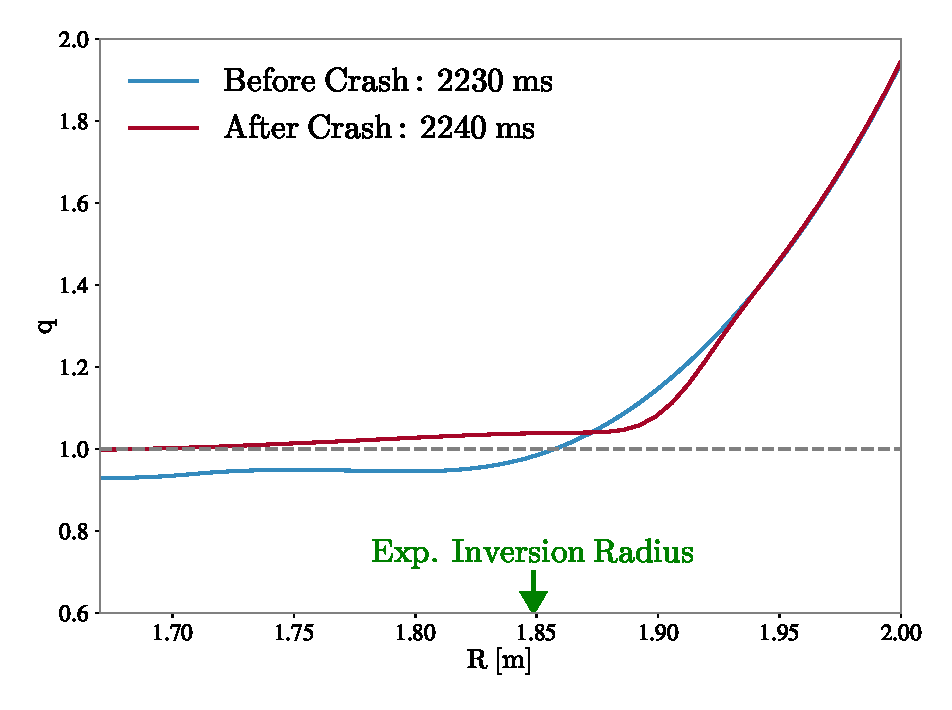
\includegraphics[width=7cm]{figures/q_profile.eps}
    }
    \subfigure[Crash Time Evolution\label{fig:sxr_crash}]{%
    	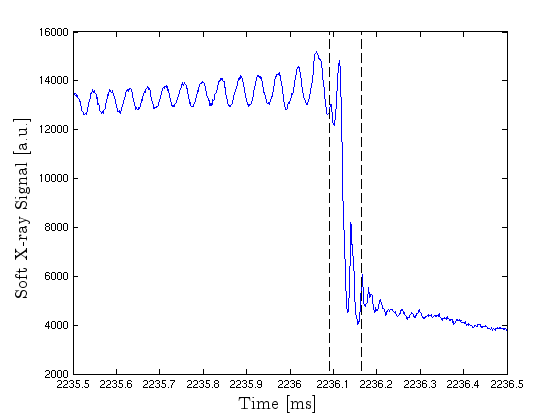
\includegraphics[width=8cm]{figures/sxr_crash.png}
    }
    \caption{(a) TRANSP calculated q profiles before (2230 ms) and after (2240 ms) the sawtooth crash. q=1 line Position of the experimental value of the inversion radius (1.85 m) is indicated in green. (b) Averaged soft x-ray signal from two poloidally similar but toroidally separated lines-of-sight. The crash occurs at 2236 ms and has a duration of approximately 75 $\mu$s indicated by the dashed vertical lines. Figure courtesy of Asger Schou Jacobsen. }
\end{figure}

We use experimental FIDA data to reconstruct the fast-ion distribution before and after the sawtooth crash. The FIDA system at ASDEX upgrade is ideal for Orbit Tomography as it has multiple radial arrays viewing the same beam from different angles, providing excellent coverage of the fast-ion phase-space. Additionally, each line of sight views both the red and blue shifted spectrum and, since ASDEX Upgrade does not use a graphite wall, the red shifted wavelengths are not corrupted by Carbon impurities, which are present in DIII-D discharges. Figure \ref{fig:augd_chords} shows the ASDEX Upgrade's FIDA systems.
\begin{figure}[h!]
    \centering
    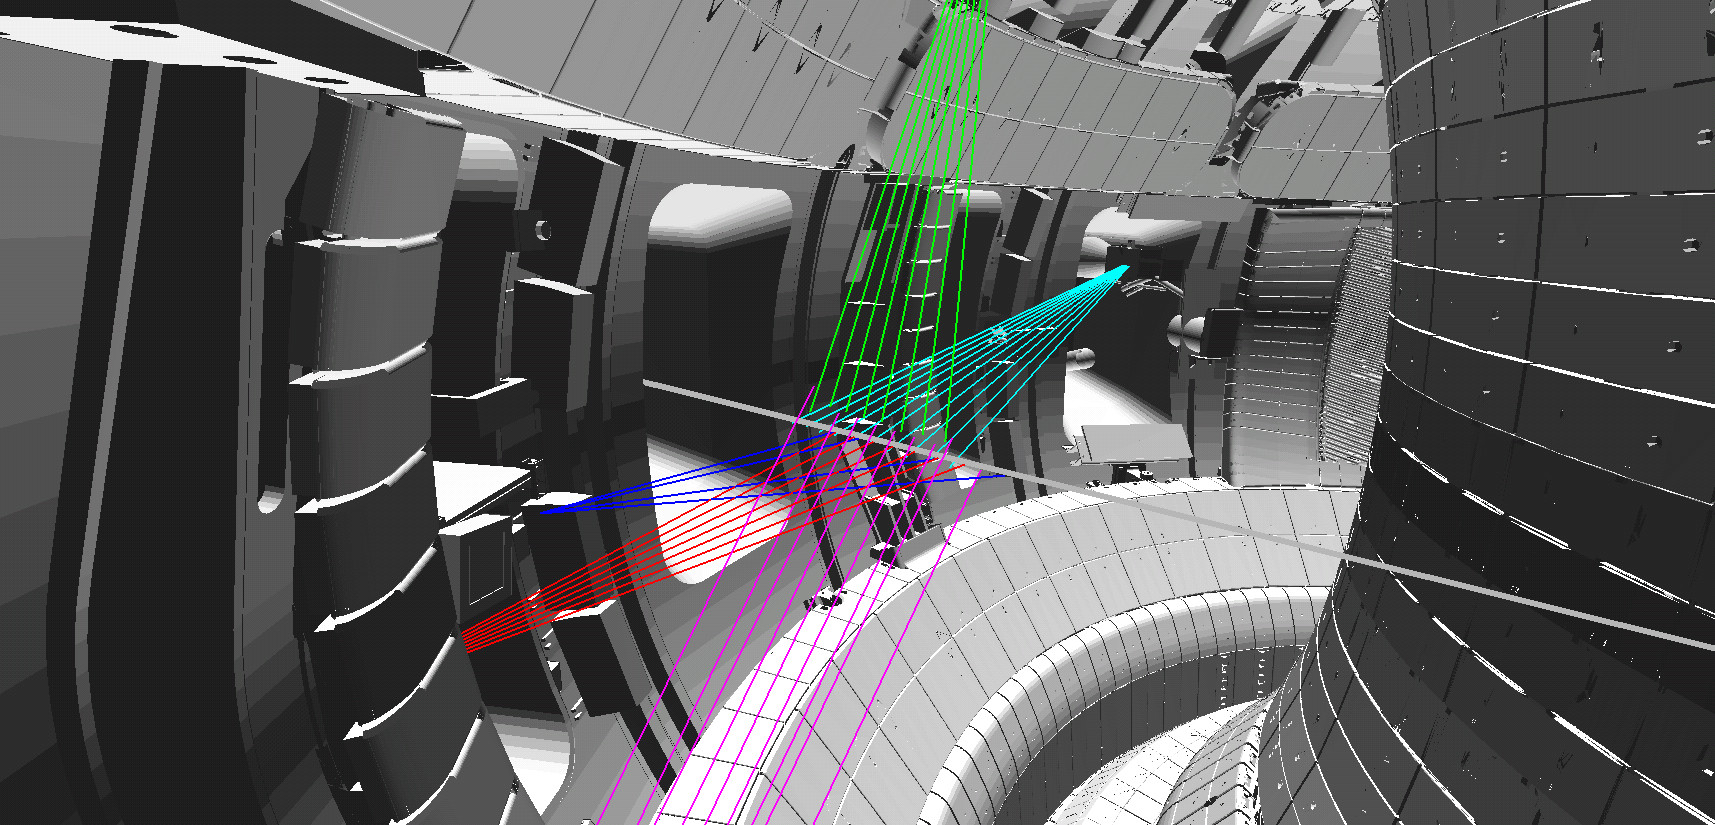
\includegraphics[width=16cm]{figures/augd_chords.jpg}
    \caption{ASDEX Upgrade FIDA lines-of-sight. 26 lines-of-sight comprising of $\sim2300$ measurements are used to reconstruct the fast-ion distribution before and after the sawtooth crash. Figure courtesy of Markus Weiland\cite{weiland2016}}
    \label{fig:augd_chords}
\end{figure}
Figure \ref{fig:augd_data} shows the experimental data, which is collected 5 ms before and after the sawtooth crash. 
\begin{figure}[h!]
    \centering
    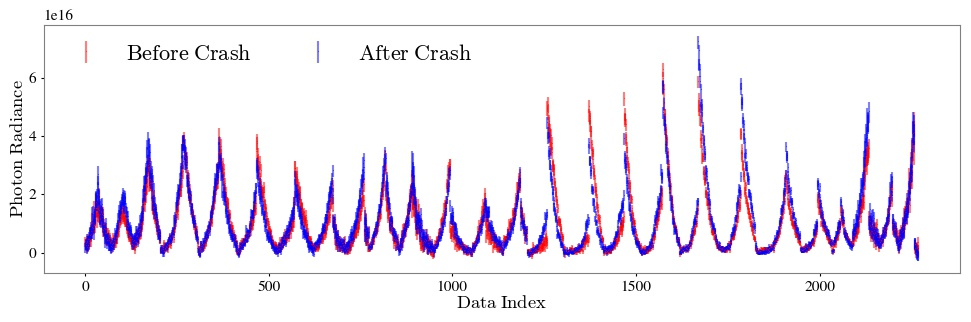
\includegraphics[width=16cm]{figures/sawtooth_data.jpg}
    \caption{ASDEX Upgrade FIDA data taken 5 ms before (red) and after (blue) the sawtooth crash.}
    \label{fig:augd_data}
\end{figure}

Despite the excellent FIDA system, some issues arose. The slowing down time of the distribution was too short. This prevented the use of time slice subtraction to remove background signal. As a consequence, a large passive FIDA signal was present in the outer lines-of-sight, a source of systematic error. To resolve the issue, the passive FIDA was included in the analysis. This was easier said than done. The calculation of the passive FIDA requires the cold edge neutral density, which is not well diagnosed. For our analysis we used the 1D neutral diffusion model implemented in TRANSP along with a scale factor that was chosen via log-evidence maximization. A similar scheme was used in analyzing passive FIDA emission in NSTX-U\cite{hao2018measurement}. Additionally, sawtooth crashes are known to impact the edge neutral density. Since the edge neutral scale factor has an inverse relationship with the fast-ion density, the inversion method could interpret this as an change in the fast-ion density at the edge. To prevent this, it is assumed that the sawtooth crash has no affect on the total number of fast ions. This is a reasonable assumption for a 59~keV beam ions at I$_p$ = 1~MA for sawteeth with a normalized inversion radius of $\rho_p$ = 0.47. This was enforced by introducing a ``measurement'' of the total number of fast ions.

\begin{figure}[h!]
    \centering
    \includegraphics[width=16cm]{figures/before_after_distributions.eps}
    \caption{Top: Reconstruction of the fast-ion distribution 5 ms before the sawtooth crash. Bottom: Reconstruction of the fast-ion distribution 5 ms after the sawtooth crash. Both distributions are on the same color scale.}
    \label{fig:before_after}
\end{figure}
In the previous study of this discharge\cite{salewski2016high}, Velocity-space Tomography was used to infer the local fast-ion distribution function within the $q=1$ surface, in which they observed a $\sim$30\% reduction in the fast-ion population most of which were passing fast-ions. Figure \ref{fig:before_after} shows the reconstructed fast-ion distributions 5 ms before and after the sawtooth crash. It can be seen in the center column that there is a depletion of fast-ions for $R_m < 1.8$ m. Figures \ref{fig:rz_diff}-\ref{fig:rz_percent_diff} show the absolute and percent differences of the reconstructions projected onto the poloidal plane. These figures show a $\sim30$\% decrease within the $q=1$ surface and a corresponding increase outside the $q=1$ surface. This is consistent with the previous analysis of this discharge as well as other experimental studies.\cite{weiland2016,du2018inpa,salewski2016high}. From these figures, it also easy to identify the inversion radius, which lies just inside the $q=1$ surface. This agrees with our previous estimate that used ECE measurements. It is also consistent with Figure \ref{fig:inpa_sawtooth}, which showed the same trend for a DIII-D discharge.
\begin{figure}[h!]
    \centering
    \subfigure[Absolute Difference\label{fig:rz_diff}]{%
    	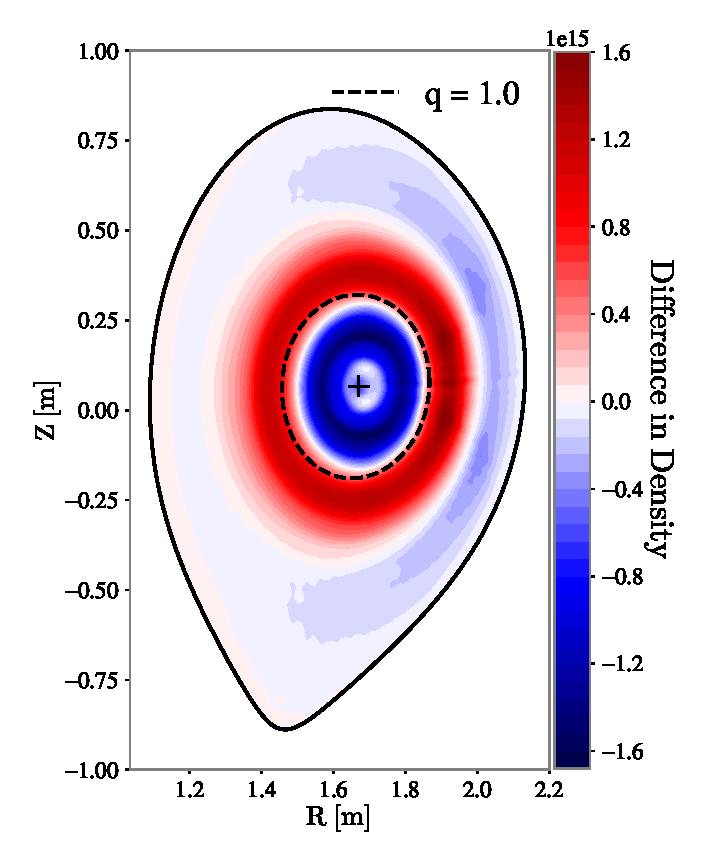
\includegraphics[width=7cm]{figures/rz_diff.eps}
    }
    \subfigure[Percent Difference\label{fig:rz_percent_diff}]{%
    	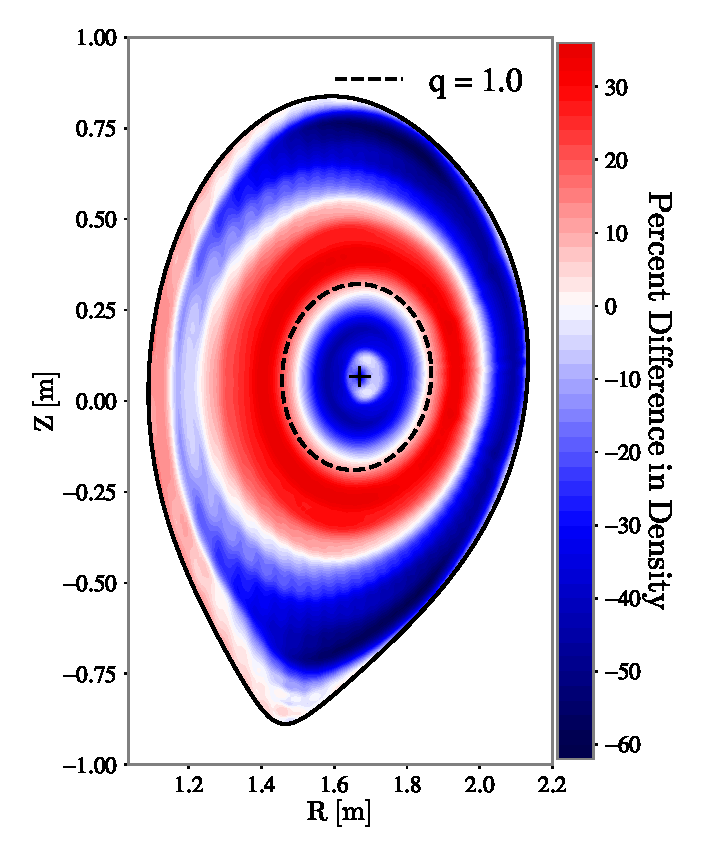
\includegraphics[width=7cm]{figures/rz_percent_diff.eps}
    }
    \caption{Experimental absolute and percent differences in fast-ion density 5 ms before and after the sawtooth crash}
\end{figure}
Since the entire fast-ion distribution function is at our disposal, we can zoom in on a specific spatial location to study local transport. Figures \ref{fig:ep_diff} show the experimental absolute and percent differences in energy-pitch space both inside and outside the $q=1$ surface. These figures \emph{again} confirm previous experimental studies since they also show that the co-passing fast-ions are the most affected by the sawtooth crash inside the $q=1$ surface (Fig. \ref{fig:ep_diff_inside}).  
\begin{figure}[h!]
    \centering
    \subfigure[Absolute Difference Inside q=1 Surface\label{fig:ep_diff_inside}]{%
    	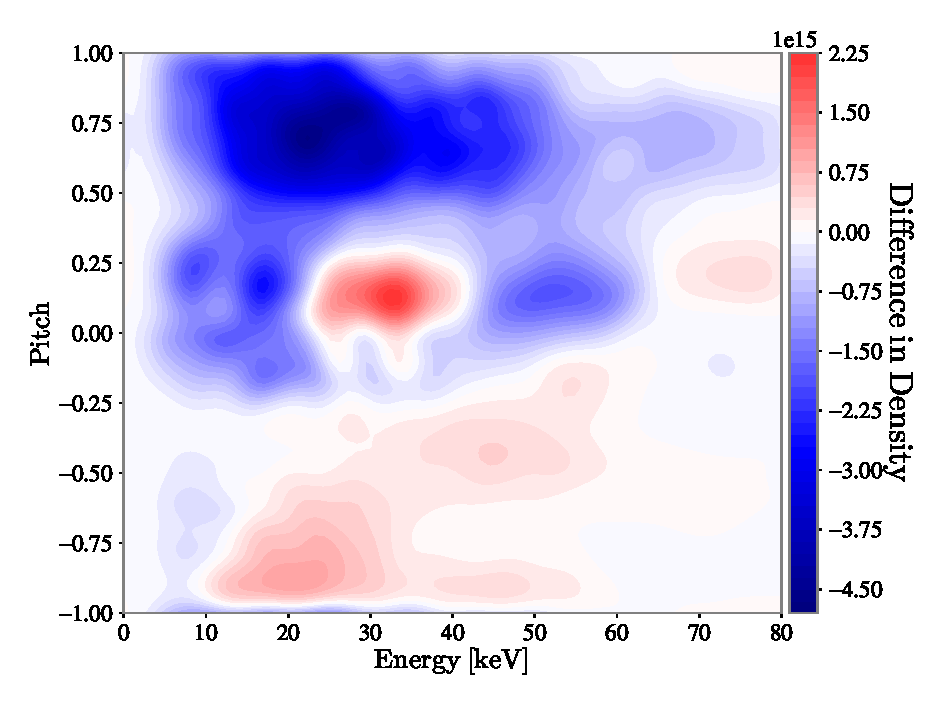
\includegraphics[width=7cm]{figures/ep_diff_inside.eps}
    }
    \subfigure[Percent Difference Inside q=1 Surface\label{fig:ep_percent_diff_inside}]{%
    	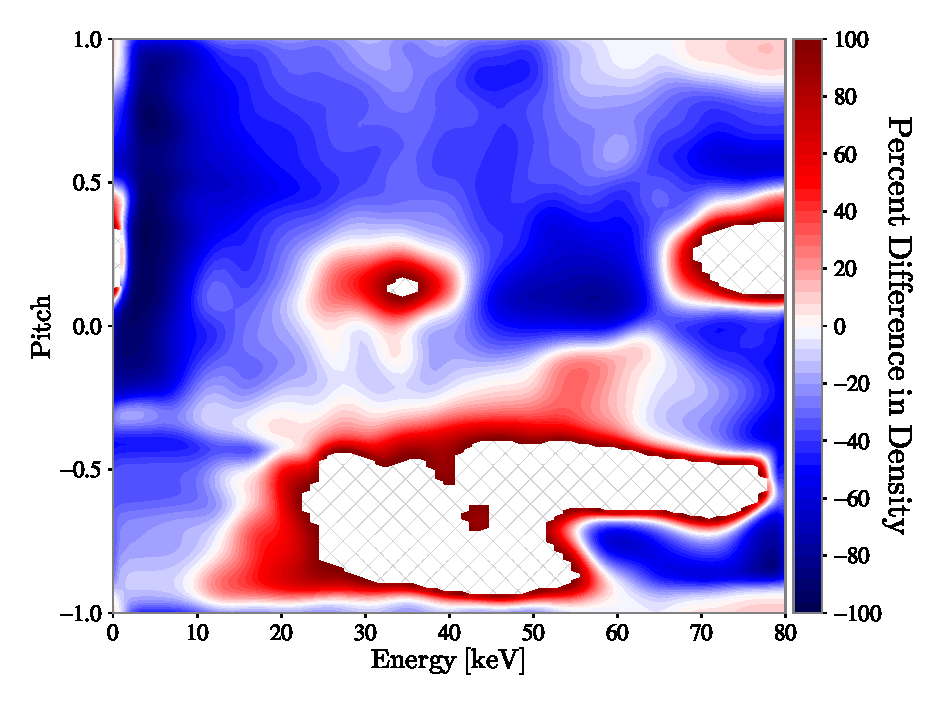
\includegraphics[width=7cm]{figures/ep_percent_diff_inside.eps}
    }
    \subfigure[Absolute Difference Outside q=1 Surface\label{fig:ep_diff_outside}]{%
    	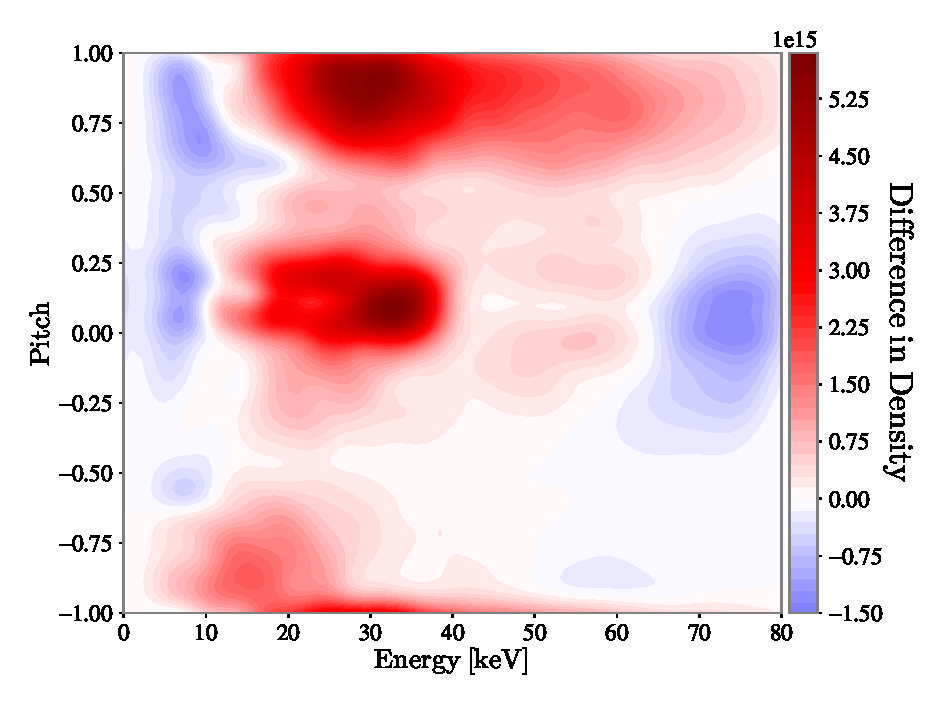
\includegraphics[width=7cm]{figures/ep_diff_outside.eps}
    }
    \subfigure[Percent Difference Outside q=1 Surface.\label{fig:ep_percent_diff_outside}]{%
    	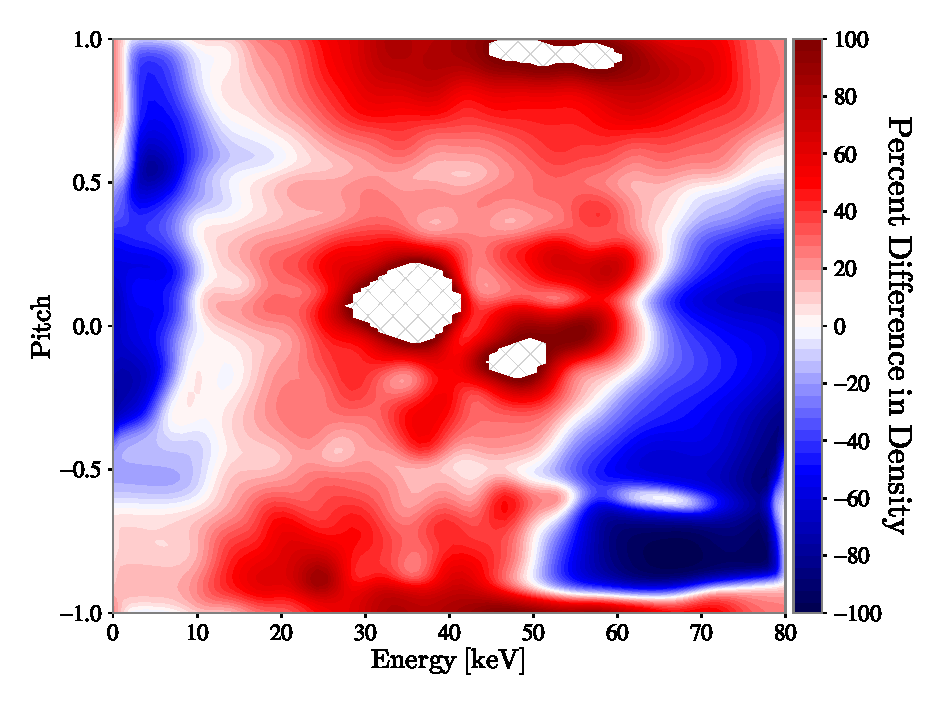
\includegraphics[width=7cm]{figures/ep_percent_diff_outside.eps}
    }
    \caption{Experimental absolute and percent differences in Energy-pitch space 5 ms before and after the sawtooth crash inside the q=1 surface at R=179 cm (top row) and outside the q=1 surface at R=191 cm (bottom row). Hatched areas are where the percent differences diverged due to a small denominator.}
    \label{fig:ep_diff}
\end{figure}

\section{Discussion}
With the validation of the results of previous sawtooth experiments, Orbit Tomography has proven itself to be a powerful new analysis technique.
Before Orbit Tomography, there was no way to \textit{know} what fast-ion distribution generated the diagnostic measurements.
The only thing that could be definitively stated was that a given theoretical distribution produces synthetic data that is consistent with all the experimental measurements.
This can lead to binary conclusions---If the synthetic data matched the experimental data then we could state that the fast-ions behaved as expected; if synthetic data \textit{didn't} match the experimental data then we could state that the fast-ions \textit{didn't} behave as expected.
With Orbit Tomography, however, the need for a theoretical distribution is negated and the fast-ion distribution can be inferred directly from the data.

For theoretical physicists, Orbit Tomography provides a way to validate their models down to the finest details.
For experimental physicists, it facilitates analysis that could only have been previously done using theoretical models.
Orbit Tomography also allows experimentalists to know, in great detail, what the knobs on the tokamak actually do to the fast-ion distribution function.
This leads to more agile development of optimized regimes---we try an experiment, we use Orbit Tomography to determine what happened to the distribution, with that information we improve the experiment. This type of iterated development could lead to the faster creation of high performance scenarios. 

In its current form, Orbit Tomography could fundamentally change fast-ion physics, however, it would not do to rest on one's laurels. In the next chapter, we look towards the future of Orbit Tomography where we discuss ways to improve the method and an exciting new application of the technique.